\subsection{Indirect remarks}
\label{sec:other}

So far, I have tried to capture one specific area of politeness phenomena: what people infer about white lies given a lay speaker's utterance. However, our model can be extended to make predictions about other kinds of polite speech. Here I focus on one additional case study: indirect remarks. Through indirect remarks, speakers try to convey a particular message in a more nuanced way. This is different from white lies, in that speaker's intentions are no longer hidden, but revealed with suboptimal efficiency. Below I present partially completed work as well as proposed research looking at production and comprehension of indirect remarks.

\subsubsection{Background and model implications} 

%Why would people speak indirectly? Theoretical accounts of indirect speech in situations of potential conflicts argue that indirect language maintains plausible deniability \citep{pinker2008}, and suggests higher stakes for the listener than speaker in case the speaker's wants are not fulfilled \citep{franke2016}. For example, a mobster trying to coerce a restaurant owner into paying protection money, who utters, ``Your daughter is very sweet. She goes to the school in Willow Road, I believe.'' avoids the risk of being sued for threat but also suggests to the owner that his stakes for not paying money are high (his daughter would be in danger). 
%
%Indirect speech in politeness situations, however, is distinguished from speech aimed upon avoiding legal liability or persuading the listener to defer to the speaker's propositions. Why would it be better to say ``I would love another glass of wine, thanks.'' than ``Pour me more wine''? The latter more clearly conveys the guest's intention for the waiter to pour more wine. But the former is less imposing on the waiter, and circumvents an impression that the speaker is in a position to give orders to the listener. Indeed, even when the implied meaning of the requests is the same, people prefer requests whose literal meanings ask for the listener's permission (``Could I ask you where Jordan Hall is?'') to those with literal meanings that assume listener's obligation to respond (``Shouldn't you tell me where Jordan Hall is?'') \citep{clark1980}. Indirect requests are complicated to manipulate for many reasons, for example due to various possible semantic forms of imperatives, and my proposed work focuses on \emph{indirect remarks} as a simpler case study.

What may lead a speaker to produce indirect remarks? An indirect remark
may be motivated by the speaker's goal to convey some face-threatening
information, while being seen as a polite person who avoids threatening
others' face. In our previous work, we described a pragmatic listener
that jointly inferred the true state and the goals of the speaker \citep{yoon2016}.
Building on this model, I describe here a speaker whose goal is to lead
this pragmatic listener to infer the true state \emph{and} attribute to
the speaker certain goals (e.g., face-saving). For instance, ``It wasn't
amazing'' does not preclude the possibility that the presentation was
bad, and may in fact be pragmatically strengthened to mean that it was
actually bad. Yet because the speaker does not choose the more direct
``It was bad'', the listener will infer a face-saving goal. Thus saying
``It wasn't amazing'' can accomplish the goal of conveying that the
presentation was bad while the speaker is seen as not wanting to make
the listener feel bad. On the other hand, if the speaker does not care
about being seen as face-saving, she will produce less indirect speech.
Further, if the presentation was actually good, or even decent, the
speaker will prefer to produce a directly positive remark (``It was
good'') in either case. Thus I predict more indirect speech when the
true state is bad, and an interaction with the speaker's desire to both
be informative and be seen as wanting to save face. 

%There have been some relevant cross-cultural evidence that people do take into account face-informativity tradeoff for polite indirect speech: 
%Hebrew adult speakers rate conventional indirect requests as more polite than direct orders or hints, and reason that both face concern and informativity are important for speech to be considered polite \citep{blumkulka1987}; 
%similarly, English and Korean adult speakers find evasive remarks to be better than direct or irrelevant remarks \citep{holtgraves1990}.
%Finally, \citet{holtgraves2016} suggested that people think of subtle utterances as reflecting varying degrees of both politeness or uncertainty (related to informativity). 
%
%Thus I hypothesize that, similar to white lies, indirect speech reflects speaker's desires to balance between the goal to be informative (convey information in the most direct manner possible) and the goal to save face, this time concerning the speaker's own face as well (maintain her reputation for conveying accurate information with intentions to be polite). In the next two subsections, I describe our extended model up to date and its empirical support, as reported in \citet{yoon2017}.


\subsubsection{Model extensions and predictions} 

Here I report extensions to our previous model up to date, 
submitted for the Cognitive Science Conference \citep{yoon2017}. 
We build on pRSA by adding negative utterances and modeling a more
sophisticated speaker. First, we extend the utterance alternatives to
include negation: The speaker may now say, \{It \emph{wasn't} terrible, bad,
okay, good, and amazing\}. These utterances indirectly address the
referent by negating certain state. We assume that it is more costly to
say utterances with negation, which makes the utterance morphemically
longer and is harder to process \citep{clark1972}. 
%In the full data
%analysis, We put a prior on this negation cost parameters and infer its
%likely values from the data.
%

Importantly, we extend the recursive reasoning in the model. For
our experiment, we consider the pragmatic speaker (\(S_2\)) who chooses
an utterance based on the pragmatic listener model, 
%(Eq. \ref{eq:L1}),
thinking about the state as well as goal weights that the pragmatic
listener will infer.
\[P_{S_2}(w \mid s, \hat{\beta})\propto \mathrm{exp}(\lambda_{2} \cdot \ln(P_{L_1}(s,  \hat{\beta} \mid w)) - C(w))\]
This crucially captures the idea that the speaker both wants to convey
the state \(s\), and to be seen as someone with goals \(\hat{\beta}\).
we simplify from the \citet{yoon2016} model by including only a single
mixture parameter \(\phi\) governing the extent to which the speaker is
being informative vs.~face saving: \(\beta_{epi} = \phi\),
\(\beta_{soc} = 1 - \phi\).

The \(S_2\) speaker in this proposed model has the goal to convey the state and to
be seen as having a particular set of goals. We explored predictions for
3 hypothetical speakers, corresponding to 3 different \(\phi\) mixture
parameter weights: (a) an \emph{informative} speaker who wants to convey
high epistemic utility (prioritizing information transfer;
\(\phi = 0.9\)) (b) a \emph{social} speaker who wants to convey high
social utility (making the listener feel good; \(\phi = 0.1\)) (c) a
\emph{both-goal} speaker who wants to convey a balance between the two
utilities (\(\phi = 0.5\)).
%\footnote{In addition, the model has a few
%  parameters not of theoretical interest. For the purposes of generating
%  model predictions \emph{a priori}, we assigned values to these
%  parameters consistent with the previous literature with this class of
%  models: the speaker optimality parameter (\(\lambda_{1}\) assigned to
%  2); the pragmatic speaker optimality parameter (\(\lambda_{2}\) to 2);
%  the value scale parameter (\(\alpha\) to 1) in the utility function;
%  and the parameter governing the cost of producing a negation (\(C(u)\)
%  to 2).}

Figure 2 (left) shows the speaker's production probabilities associated %fixme:figure
with producing an indirect speech act (i.e., an utterance with negation)
for the three different speakers as the true state of the world is
varied. We see, consistent with the intuition, that indirect speech was
relatively more preferred in bad states than in good states. As well, we
see higher probability of negation production for the speaker who wants
to convey both goals (epistemic and social) relative to each goal
independently. Indirect speech does not convey that much information and
so the informative speaker (a) would disprefer it. The social speaker
(b) who wants to convey a face-saving goal would tend to signal a
better-that-actual state through direct positive remarks. The both-goal
speaker produces indirect remarks to avoid direct remarks that are
either true but face-threatening, or face-saving but false.

\begin{CodeChunk}
\begin{figure*}[t]

{\centering 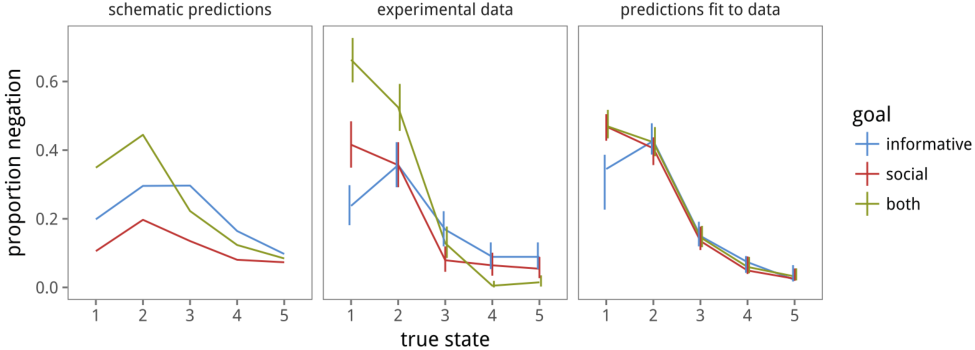
\includegraphics{figures/exptModelNeg-1} 

}

\caption{Schematic model predictions (left), Experiment 1 results (center) and fitted model predictions (right) for average proportion of negation produced among all utterances, given true states (x-axis) and goals (colors).}\label{fig:model_pred_negNoneg}
\end{figure*}
\end{CodeChunk}

\subsubsection{Empirical test: Experiment 1} 

\paragraph{Procedure}

To compare against the model predictions, we ran the first experiment to measure participants'
predictions for the most likely utterance (\(w\)) produced by the
speaker, given a description of the true state. For example, given that
Ann wanted to make Bob feel good but felt that his poem deserved 2 out
of 5 hearts, what would she say? 
%I hypothesized that when there was no
%tradeoff between informativity and face-threat avoidance (i.e., when the
%addressee's performance was great), speakers would use truthful and
%face-saving direct remarks (``{[}Your poem{]} was amazing'') regardless
%of their described goals. However, when there was a conflict between the
%epistemic and social goals (i.e., when the addressee's performance was
%poor), a speaker who tried to convey both goals would use vague indirect
%remarks (``{[}Your poem{]} wasn't terrible'') more often than direct
%face-threatening remarks (``{[}Your poem{]} was bad''; preferred by a
%speaker who only considered the epistemic goal) or direct face-saving
%remarks (``{[}Your poem{]} was good''; preferred by a speaker who wanted
%to convey only a social goal).
We presented the same context items as Experiment P1-2 and provided information on the speaker Ann's goal -- \emph{to make Bob feel good},
or \emph{to give as accurate and informative feedback as possible}, or
both -- and the true state -- how Ann actually felt about Bob's
performance (e.g., 2 out of 5 hearts). 
Each scenario was followed by a question that read, ``If Ann wanted
\emph{to make Bob feel good} but not necessarily give informative
feedback (or \emph{to give accurate and informative feedback} but not
necessarily make Bob feel good, or \emph{BOTH make Bob feel good AND
give accurate and informative feedback}), what would Ann be most likely
to say?'' Participants indicated their answer by choosing one of the
options on the two dropdown menus, side-by-side, one for choosing
between \emph{was} vs. \emph{wasn't} and the other for choosing among
\emph{terrible}, \emph{bad}, \emph{okay}, \emph{good}, and
\emph{amazing}.\footnote{The experiment can be viewed at: \url{https://langcog.stanford.edu/expts/EJY/polgrice/speaker_production_dropdown_v2/speaker.html.}}
%
%\begin{CodeChunk}
%\captionsetup{width=0.8\textwidth}
%\begin{figure}[h]
%{\centering 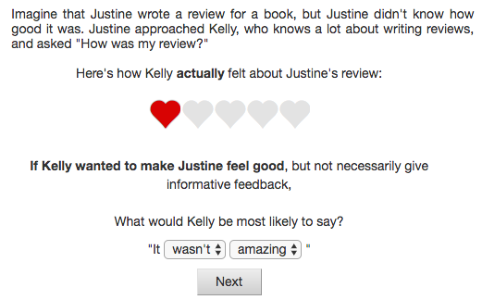
\includegraphics{figures/expt_screen-1} 
%
%}
%
%\caption[Example of a trial in Experiment 1]{Example of a trial in Experiment 5.}\label{fig:expt2_screen}
%\end{figure}
%%\begin{wrapfigure}{L}{0.5\textwidth}
%%  \begin{center}
%%    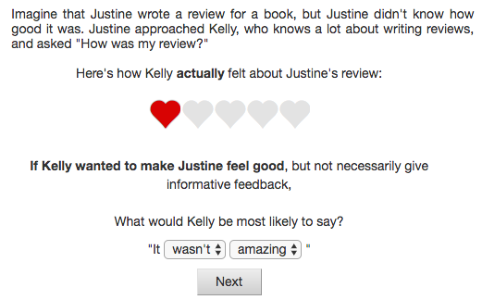
\includegraphics[width=0.48\textwidth]{figures/expt_screen-1}
%%  \end{center}
%%  \caption{Example of a trial in Experiment 5.}\label{fig:expt2_screen}
%%\end{wrapfigure}
%\end{CodeChunk}




\paragraph{Findings}

Our hypotheses for utterance production by speakers with different goals
were borne out. Speakers with both
informative and social goals produced more indirect remarks than were
observed in the other two goal conditions (Figure 2, center). 
Our extended model explained almost all of the variance in the
average data \(r^2\)(15) = 0.962. 

However, while the model in the \emph{both} condition did produce indirect
utterances (e.g. ``It was not terrible'' given 1 heart) it did so
slightly less than the empirical data. For this reason, the model did
not yield the expected difference for negation production between
both-goal and social conditions (Figure 2, right). 
These deviations are to be examined further,
by looking into possible different discrepancies between the model and experimental paradigm, 
and possible alternative models for simulating the pragmatic speaker 
(e.g. varying whether she only cares about her self-representation goals, 
or also has genuine goals to be informative considerate).

\subsubsection{Empirical test: Experiment 2} Whereas Experiment 1 looked at the speaker production, I will also look at listener inferences. I will use tasks identical in design to Experiments P1-2, but looking at indirect speech instead of white lies. I will test participants' judgments in contexts in which Bob asks Ann for her opinion on his cookie. I hypothesize that participants will attribute more niceness but less informativity to Ann when she says ``It wasn't amazing,'' compared to ``It was terrible.'' This will show that indirect remarks are similar to white lies and reflect speakers' consideration of face-informativity tradeoff.





%%% Local Variables: 
%%% mode: latex
%%% TeX-master: "desc"
%%% End

